
%%%%%%%%%%%%%%%%%%%%%%%%%%%%%%%%%%%%%%%%%%%%%%%%%%%%%%%%%%%%%%%%%%%%%%%%%%%%%%%%
\chapter{Theory}
\label{chap:Theory}
\vspace{2cm}
\section{Liquid Crystals}
\label{sec:liquidcrystals}
In nature, there are a lot of materials that do not exhibit a single phase transition between the liquid and solid states, but rather a variety of so-called mesophases. In these mesophases, the materials exhibit some properties common to liquids, and some properties found in crystals. These materials are therefore aptly called liquid crystals.

For the mesophases to occur the molecules the material is made of must be anisotropic in shape. The exact properties of the different phases that the materials display are highly dependent on the molecular structure and properties, i.e., the symmetries it possesses. The most common shapes for the molecules are rod-like, in which case they are called calamitic, or disc-shaped, in which case they are called discotic. Of particular interest in this work are the discotic liquid crystals, which we discuss in more detail in the next section.

The phase transitions can occur as a function of the temperature. In this case, the liquid crystal is called thermotropic. Lyotropic liquid crystals require the presence of a solvent and exhibit phase transitions as a function of the concentration of the solvent. The liquid crystals considered in this work are thermotropic.

\subsection{Discotic Liquid Crystals}
Discotic liquid crystals are composed of disc-like molecules. As such, the molecules possess a cylindrical symmetry ($D_{\infty h}$ in Schönflies notation), i.e., the molecule has an orientational axis about which it is rotationally invariant, and is also invariant under reflections across the isotropic plane to which the orientational axis is perpendicular. We refer to this axis as the orientation of the molecule and describe it using the (unit) vector $\hat{\mathbf{e}}$ with the equivalence relation $\hat{\mathbf{e}}\sim-\hat{\mathbf{e}}$. 
In the following sections we give brief descriptions and illustrations of the phases assumed by the discotic liquid crystals investigated in this work.
\subsubsection{Isotropic Phase}
\begin{figure}[H]
 \centering
 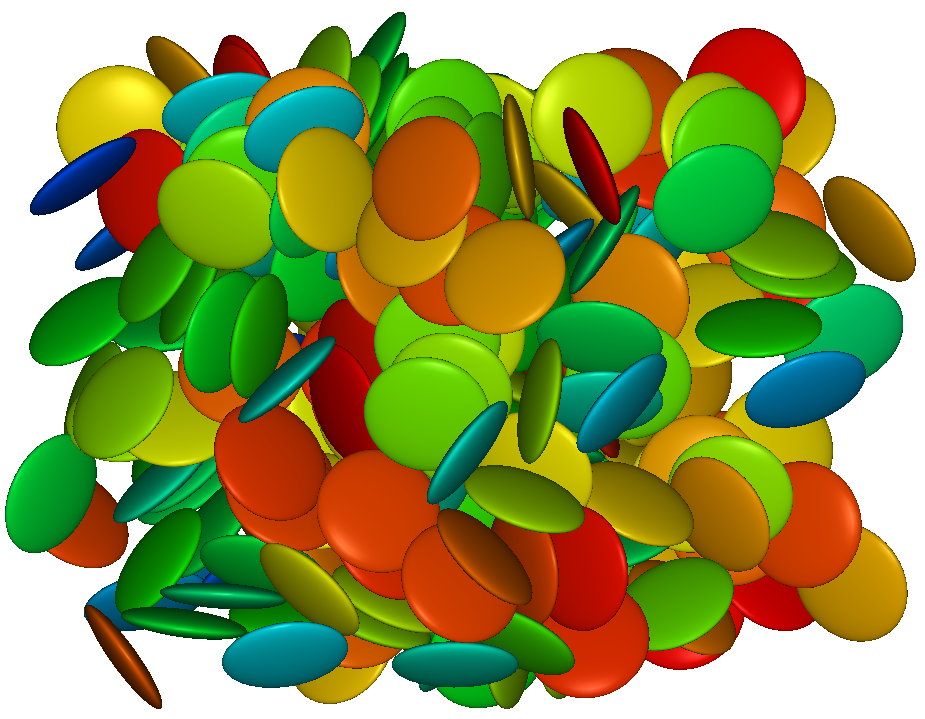
\includegraphics[width=.3\linewidth]{images/isotropic.png}
 \caption{Isotropic phase. Images are from bulk simulations at different temperatures and are visualized with the software QMGA \cite{qmga}.}
 \label{fig:isotropic}
\end{figure}

As the name suggests this phase is characterized by the isotropy of the system, that is, there is no orientational correlation between the molecules. There are however, as opposed to an ideal gas, short range spatial correlations as found in any other fluid.
\subsubsection{Nematic Phase}
\begin{figure}[H]
 \centering
 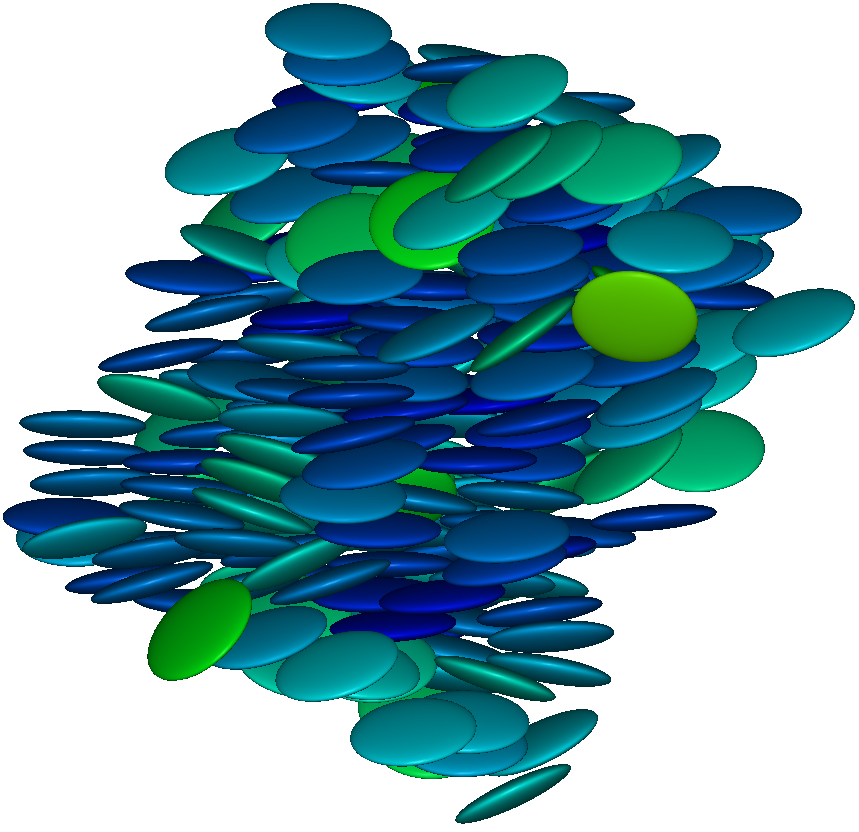
\includegraphics[width=.3\linewidth]{images/nematic.png}
 \caption{Nematic phase}
 \label{fig:nematic}
\end{figure}
The characteristic property of the nematic phase is that while there are no long range spatial correlations between the molecules, there is a distinct orientational preference, i.e. the particles are mostly aligned along a specific direction, represented with a vector called the director $\hat{\mathbf{n}}$. The system remains invariant under rotations around $\hat{\mathbf{n}}$. The phase therefore possesses a $D_{\infty h}$ symmetry.
\subsubsection{Columnar Phase}
\begin{figure}[H]
 \centering
 \subfigure[Seen from the side\label{fig:columnarside}]
   {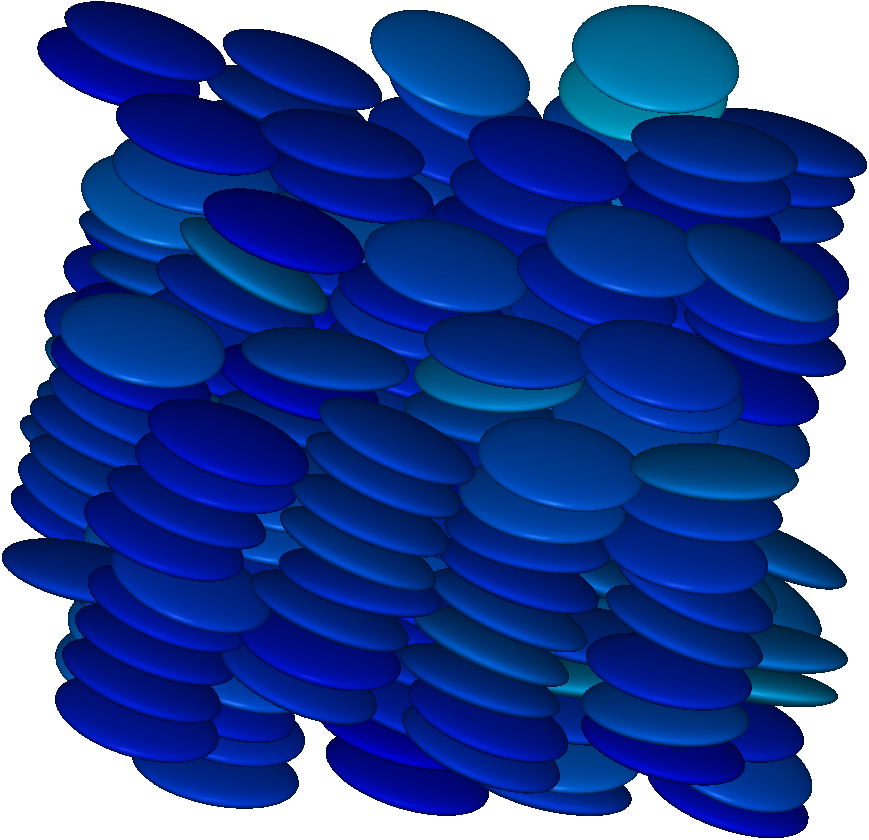
\includegraphics[width=0.3\textwidth]{images/columnar.png}}
\subfigure[Seen from above\label{fig:columnarabove}]
   {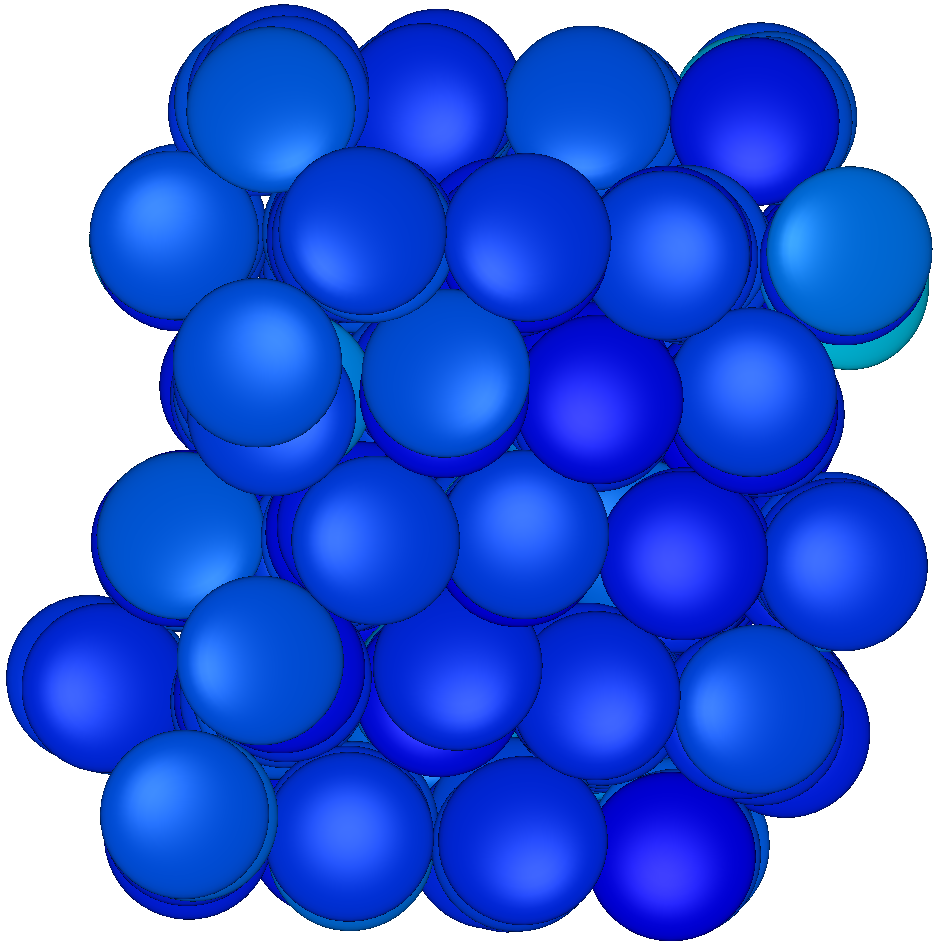
\includegraphics[width=0.3\textwidth]{images/columnarabove.png}}
 \caption{Columnar phase}
\end{figure}

At lower temperatures, molecular interactions favor an arrangement where the molecules stack on top of each other, and thus long columns in one direction emerge. The columns arrange themselves in a hexagonal lattice, since the highest-density configuration for circles in 2-D planes is the hexagonal packing arrangement \cite{chang2010simple}. 
The system is liquid in one dimension, along the columnar axis, and solid in the other two.
This phase possesses a $D_{6 h}$ symmetry.
\subsubsection{Crystal Phase}
\begin{figure}[H]
 \centering
 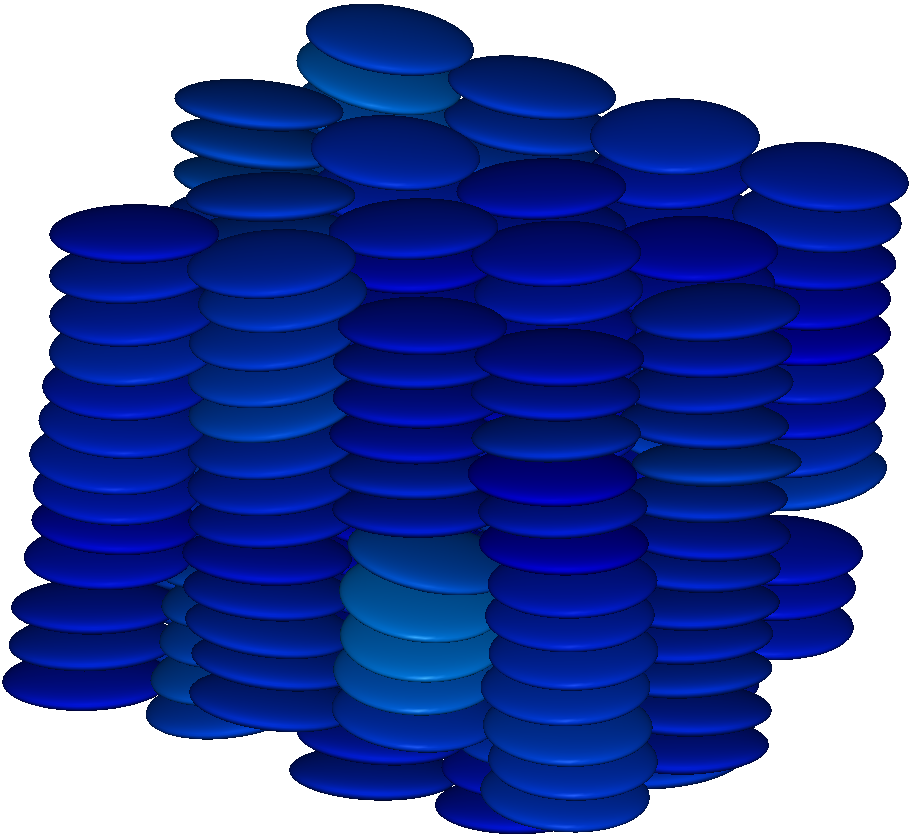
\includegraphics[width=.3\linewidth]{images/crystal.png}
 \caption{Crystal phase}
 \label{fig:Crystal phase}
\end{figure}
Upon further cooling, the individual columns solidify, creating a body-centred orthorhombic crystal phase.

\subsubsection{Confined Phases}
\label{subsubsec:confinedphases}
By restricting the geometry of the liquid crystal system one can favor certain phases, shifting the phase diagram, and create new configurations entirely \cite{zhang2015columnar,sentker2018quantized}.
A confining wall will induce a preferential alignment of the liquid crystal molecules at its surface, because of physical and chemical interactions. We call this preferential alignment `anchoring'.
In particular, by confining the system to a cylindrical shape and enforcing a circular edge-on anchoring of the particles to the outer wall, i.e, by favoring an alignment of the molecules near the wall perpendicular to both the radial position and the cylindrical axis, one can observe the quantized appearance of concentric columnar rings. Starting from the wall, the annular layers propagate inward layer-by-layer discretely. 
\begin{figure}[H]
 \centering
 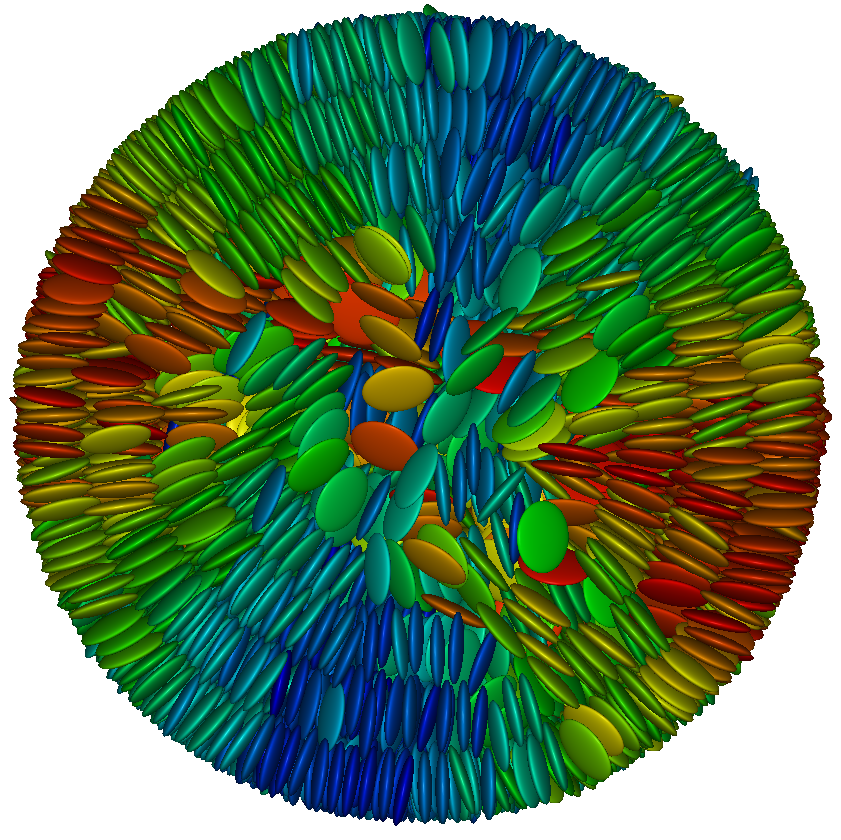
\includegraphics[width=.3\linewidth]{images/confined.png}
 \caption{Concentric columnar rings arising due to the cylindrical confinement. \cite{sentker2018quantized}}
 \label{fig:pore}
\end{figure}


\subsection{Order parameters}
\label{subsec:orderparameters}
The goal of this subsection is to define a suitable order parameter with which we can describe the phase transitions of the given liquid-crystal system.

\subsubsection{Nematic order parameter}
We can study many physical properties of a given material by their reaction to a (small) perturbation such as an electric or magnetic field. Our goal is to define an orientational order parameter. Therefore it is sensible to consider the orientation of both the perturbation and the reaction. Given a perturbation $P_\beta$, we can write the reaction $R_\alpha$ as
\begin{align*} 
    R_\alpha = {R_0}_\alpha + \displaystyle\sum_\beta\chi_{\alpha\beta} P_\beta + \displaystyle\sum_{\beta,\chi}\chi_{\alpha\beta\gamma} P_\beta P_\gamma + ...
\end{align*}
The physical properties of the material are encoded in the coefficients $\chi_{\alpha\beta},\, \chi_{\alpha\beta\gamma},\,...$. An orientational order parameter should describe how much the system deviates from an isotropic state. A good ansatz is thus to take the second order tensor $\chi_{\alpha\beta}$ and extract the isotropic part. This tensor can be represented by a $3\!\times\!3$ matrix, which we shall denote by $\chi$.

Because of the $D_{\infty h}$ symmetry of the discotic liquid crystal molecule, the matrix takes the form
\begin{align}
   \chi = \begin{pmatrix}
    \chi_\perp&0&0\\
    0&\chi_\perp&0\\
    0&0&\chi_\parallel
    \end{pmatrix}
\end{align}
in the coordinate system where the orientation of the LC molecule is given by $\hat{\mathbf{e}}=(0,0,1)^T$.
In any other reference frame the matrix is then given by $\chi' \equiv R\chi R^{-1}$, where $R$ is the rotation matrix to that reference frame. Since we wish to define a parameter that vanishes when the material is completely isotropic and is 1 when it is fully aligned, we need to extract the isotropic component of the matrix, given by  $\frac{\mathrm{tr}(\chi)}{3}\id$ . Therefore we find that  $\chi' - \frac{\mathrm{tr}(\chi)}{3}\id$ is the anisotropic part of the tensor $\chi'$. Let's consider explicity $\chi' - \frac{\mathrm{tr}(\chi)}{3}\id$ :
\begin{align*}
    \chi' - \frac{\mathrm{tr}(\chi)}{3}\id &= R\chi R^{-1} - \frac{\mathrm{tr}(\chi)}{3}\id \\
                                           &= R (\chi - \frac{\mathrm{tr}(\chi)}{3}\id) R^{-1} \\ 
                                           &= R \left(\frac{1}{3}\left(3  
    \begin{pmatrix}
    \chi_\perp&0&0\\
    0&\chi_\perp&0\\
    0&0&\chi_\parallel
    \end{pmatrix}
    -
    \begin{pmatrix}
    2\chi_\perp+\chi_\parallel&0&0\\
    0&2\chi_\perp+\chi_\parallel&0\\
    0&0&2\chi_\perp+\chi_\parallel
    \end{pmatrix}\right)\right)R^{-1}\\
    &= R \left(\frac{1}{3} 
    \begin{pmatrix}
    \chi_\perp-\chi_\parallel&0&0\\
    0&\chi_\perp-\chi_\parallel&0\\
    0&0&2(\chi_\perp-\chi_\parallel)
    \end{pmatrix}
    \right)R^{-1} \\
    &=  \Delta \chi \, R \left( 
    \begin{pmatrix}
    0&0&0\\
    0&0&0\\
    0&0&1
    \end{pmatrix}
    -\frac{1}{3}
    \begin{pmatrix}
    1&0&0\\
    0&1&0\\
    0&0&1
    \end{pmatrix} \right)
    R^{-1},  \qquad \text{where }\Delta \chi= \chi_\parallel - \chi_\perp \\ 
    &= \Delta \chi (R (\hat{\mathbf{e}} \otimes \hat{\mathbf{e}} - \frac{1}{3} \id)R^{-1}) \\
    &= \Delta \chi (R (\hat{\mathbf{e}}\otimes \hat{\mathbf{e}}) R^{-1} - \frac{1}{3} \id) \\
    &= \Delta \chi (\hat{\mathbf{e}'}\otimes \hat{\mathbf{e'}} - \frac{1}{3} \id).
\end{align*}
We can therefore define the nematic order parameter is the average normalized anisotropy over the entire system $Q \equiv \langle \frac{3}{2}(\hat{\mathbf{e}'}\otimes \hat{\mathbf{e'}} - \frac{1}{3} \id )\rangle$. The scalar order parameter $S$ is defined as the largest eigenvalue\footnote{This is well-defined, since $Q$ is a symmetric matrix. By the principal axis theorem $Q$ has three real eigenvalues, in particular a largest eigenvalue.} of $Q$ and the director $\hat{\mathbf{n}}$  as the corresponding eigenvector.
This definition allows some insight into the nature of the scalar order parameter. Keeping the same notation we have
\begin{align*}
    S &= S \hat{\mathbf{n}}^T \hat{\mathbf{n}}    \\
      &= \hat{\mathbf{n}}^T Q \hat{\mathbf{n}}\\
      & = \langle \hat{\mathbf{n}}^T \frac{3}{2}  (\hat{\mathbf{e}}\otimes \hat{\mathbf{e}} - \frac{1}{3} \id) \hat{\mathbf{n}}\rangle\\
      &=  \frac{3}{2}  \langle (\hat{\mathbf{n}}^T \hat{\mathbf{e}}) (\hat{\mathbf{e}}^T \hat{\mathbf{n}}) - \frac{1}{3} \rangle\\
      &=   \langle \frac{1}{2}( 3\cos^2(\theta) - 1) \rangle \\
      &=   \langle P_2(\cos(\theta)) \rangle , \quad  P_2(x)= \frac{1}{2}( 3x^2 - 1).
\end{align*}
$P_2$ is the second Legendre polynomial, which corresponds to a quadrupolar symmetry, and the angle brackets indicate an ensemble average. We therefore conclude that the corresponding phase possesses a quadrupolar symmetry.
\subsubsection{Hexagonal order parameter}
In order to classify the columnar phase one needs to define an order parameter. The columnar phase is characterized by a 2D hexagonal lattice, therefore the hexagonal order parameter can be defined as
\begin{align}
    \Psi_6 = \left\langle \frac{1}{N} \displaystyle\sum^N_{i=1}  \frac{1}{|n_i|}\displaystyle\sum_{k,l\in n_i} \exp(6i \theta_{kl})  \right\rangle,
\end{align}
where $n_i$ denotes the particles in the immediate neighbourhood of the particle $i$. The angle $\theta_{kl}$ is calculated by taking the angle between the intermolecular vectors $\hat{\mathbf{r}}_{ik},\,\hat{\mathbf{r}}_{il}$ projected onto the plane orthogonal to the orientation vector $\hat{\mathbf{e}}_i$. The neighbourhood of the particle $i$ is defined as a thick annulus around $i$, whose thickness is $1.5\sigma_{\text{ff}}$ (see Section \ref{subsec:potentials}) and with an inner-ring radius of $0.5\sigma_{\text{ee}}$ and an outer-ring radius of $1.5\sigma_{\text{ee}}$. 
\subsubsection{Radial Distribution function}
Crystals are characterized by their light-scattering behaviour. In X-ray diffraction experiments, crystals exhibit strongly pronounced Bragg-peaks. The scattering spectrum is mathematically described by the structure factor
\begin{align}
    S(\mathbf{k}) = 1 + \int_V \exp(i \mathbf{k\cdot r})(g(\mathbf{r})-1) \text{d}\mathbf{r},
\end{align}
where $g(\mathbf{r})$ is called the pair correlation function\cite{allen1987computer}, defined as
\begin{align}
\label{eq:paircorrelation}
    g(\mathbf{r}) = \left\langle\frac{V}{N^2} \displaystyle\sum_i\displaystyle\sum_{i\neq j} \delta(\mathbf{r}-\mathbf{r}_{ij})\right\rangle,
\end{align}
where $\mathbf{r}_{ij}$ is the distance between two particles $i$ and $j$. In numerical applications, the Dirac delta distribution $\delta$ is replaced by a function which is non-zero in a small interval, thus essentially creating a histogram of pair separations in that range\footnote{Note that to normalize the histogram bins, one has to divide Eq. (\ref{eq:paircorrelation}) by the volume of the chosen interval}. The pair correlation function thus describes the probability of finding a particle at distance $\mathbf{r}$ from a reference particle. 

Since a system in an isotropic liquid phase has non-trivial short-term particle correlations the pair correlation function will not be constant, as opposed to an ideal gas for example. However, due to the isotropy of the system, it will be independent of the direction of the distance.

For a non-isotropic fluid that possesses a nematic phase, the pair correlation function will be different in the directions perpendicular to the director and the direction parallel to it. Based on Eq. (\ref{eq:paircorrelation}) one therefore can define two pair distribution functions as 
\begin{align}
    g_{\perp}(r) = \left\langle \frac{V}{N^2} \displaystyle\sum_i\displaystyle\sum_{i\neq j} \delta(r-r_{ij}^\perp)\theta\left(\sigma_{\text{ff}}-r_{ij}^\parallel\right) \right\rangle, \\
    g_{\parallel}(r) = \left\langle \frac{V}{N^2} \displaystyle\sum_i\displaystyle\sum_{i\neq j} \delta(r-r_{ij}^\parallel)\theta\left(\frac{\sigma_{\text{ee}}}{2}-r_{ij}^\perp\right)\right\rangle.
\end{align}
The components of the distance vector between two particles are
\begin{align*}
    \mathbf{r}_{ij}^\parallel &= \left(\mathbf{r}_{ij}\cdot\hat{\mathbf{e}}_i\right)\hat{\mathbf{e}}_i,\\
    \mathbf{r}_{ij}^\perp &= \mathbf{r}_{ij} - \mathbf{r}_{ij}^\parallel.
\end{align*}
The Heaviside function $\theta$ ensures a slicing of the space into sheets with thickness $2\sigma_{\text{ff}}$ and a column with diameter $\sigma_{\text{ee}}$ respectively.

Both the columnar and crystal phases exhibit sharp peaks in the perpendicular pair correlation at the positions of a hexagonal lattice, i.e., for $r_{\perp} \in \{ \sqrt{1+n+n^2}: n \in \mathbb{N}\}$. Since in the columnar phase, the particles in the columns behave like a one-dimensional liquid, the parallel pair correlation $g_\parallel$ will only show the short term correlations present in a liquid, whereas in the crystal phase it will exhibit the sharp peaks characteristic of crystals.

\subsubsection{Local order parameters}
In complex geometries, a global orientation of the particles may never occur and therefore investigating order parameters locally is necessary. In this section we will briefly present a few order parameters with which we can investigate the local structure.
\paragraph {Local nematic order parameter}

The local nematic order parameter is calculated by averaging the nematic order at a neighbourhood $n_i$ of a particle $i$ over every particle.

\begin{align}
    S_L = \frac{1}{N}\displaystyle\sum_{i=1}^N  S(n_i)
\end{align}

The neighbourhood $n_i$ of the particle $i$ is taken to be a sphere of radius $\sigma_{ee}$ around it.

\iffalse
\subsubsection{Radial density}


$\rho(r) = (1/\pi r^2 h) (1/N) \sum_i \delta (r_i-r)$


\fi
\paragraph{Averaged bond order parameter}

When investigating the local molecular order, we use the spatially resolved average local bond order parameter $\overline{q}_l(i)$ as introduced by Lechner and Dellago \cite{lechner2008accurate}. The average local bond order parameter of the $i$-th particle is thus defined as
\begin{align}
\overline{q}_l(i) = \sqrt{\frac{4 \pi}{2l+1}\displaystyle\sum_{m=-l}^{l} \left|\overline{q}_{lm}(i)\right|^2}
\end{align}
where
\begin{align}
\overline{q}_{lm}(i) = \frac{1}{|\Tilde{N}_b(i)|} \displaystyle\sum_{k\in \Tilde{N}_b(i) } q_{lm}(k),
\end{align}

and the local orientational order $q_{lm}(i)$ is

\begin{align}
    q_{lm}(i) = \frac{1}{|N_b(i)|} \displaystyle\sum_{j\in \Tilde{N}_b(i) } Y_{lm}(r_{ij}),
\end{align}
where $N_b(i)$ is the set of nearest neighbours excluding $i$ and $\Tilde{N}_b(i)=N_b(i) \cup {i}$. Using this order parameter we can determine  locally with high accuracy whether a particle is in a crystal or a liquid.



\section{Computational Methods}
\label{sec:compmethods}
Some physical systems are too complex to allow an analytical solution. In these cases computer simulations allow us to numerically study these systems and gain valuable insights. In this section we shall present a brief introduction to the theory behind the computational methods used in this work.

In statistical mechanics, one calculates an observable macroscopic property $A$ by integrating over the the phase space, i.e., the space of all possible configurations $\Gamma$
\begin{align}
\label{eq:observableexpectedvalue}
\langle A\rangle = \int \rho\left(\Gamma\right)  A\left(\Gamma\right) \mathrm{d}\Gamma
\end{align}
given the probability distribution $\rho$ of the system. Even when the solution for the probability distribution is known, the phase space usually has too high a dimensionality to exactly calculate the integral in Eq.(\ref{eq:observableexpectedvalue}). One method to solve this is to generate samples with the probability $\rho$ and calculate the average of $A$ over the samples, since for a sufficiently high number of samples
\begin{align*}
    \langle A\rangle_{\text{samples}}\equiv\frac{1}{N} \displaystyle\sum_{i=1}A(\Gamma_i) \approx \int \rho\left(\Gamma\right)  A\left(\Gamma\right) \mathrm{d}\Gamma =\langle A\rangle.
\end{align*}
To produce the samples one can use the Metropolis algorithm, which shall be presented in the next section.

\subsection{Metropolis Algorithm}
\label{subsec:metropolisalgorithm}
We begin by defining some important concepts in the derivation of the algorithm. Given a stochastic process, a Markov chain is a sequence of stochastic variables, with the property that the state of each stochastic process is only dependent on the state immediately preceding it.
Two states $\Gamma_n,\, \Gamma_m$ are linked by the probability $\pi_{mn}$, i.e. the probability that given $\Gamma_n$, the next outcome will be $\Gamma_m$. Given a probability distribution $\boldsymbol{\rho} = (\rho_1,...,\rho_n) $ for a state space $\{\Gamma_1,....\Gamma_n\}$ the probability that the next outcome is $\Gamma_m$ will be 
\begin{align}
\label{eq:markovmatrixmultiplication}
\rho_m' = \displaystyle\sum_i \pi_{mi} \rho_i.
\end{align}
Treating $\mathbb{\rho}$ as a vector, Eq. (\ref{eq:markovmatrixmultiplication}) becomes the well known multiplication of $\boldsymbol{\rho}$ by a matrix $\boldsymbol{\pi}$ which is called the transition matrix of the Markov process.
The time evolution of the system with a starting distribution $\boldsymbol{\rho}$ is given by the repeated multiplication of $\boldsymbol{\pi}$ with $\boldsymbol{\rho}$. An important result of the Markov chain theory is that (given some conditions on $\boldsymbol{\pi}$ \cite{grimmett2001probability,allen1987computer}) any starting distribution $\boldsymbol{\rho'}$ will converge to the limiting distribution $\boldsymbol{\rho}$, i.e. that $\displaystyle\lim_{n\to \infty} \boldsymbol{\pi}^n \boldsymbol{\rho'} = \boldsymbol{\rho}$. The limiting distribution then obviously satisfies 
\begin{align}
    \label{eq:limitingditributioneigenvectors}
    \boldsymbol{\rho} = \boldsymbol{\pi} \boldsymbol{\rho} \qquad \text{or} \qquad \rho_n = \displaystyle\sum_m \pi_{nm} \rho_m.
\end{align}
The goal is therefore to construct a matrix $\boldsymbol{\pi}$ such that the limiting distribution is the desired one. The method proposed by Hastings \cite{hastings1970monte} was to replace the eigenvalue equation (\ref{eq:limitingditributioneigenvectors}) by the stronger condition of detailed balance
\begin{align}
    \label{eq:detailedbalance}
    \pi_{mn} \rho_n = \pi_{nm} \rho_m.
\end{align}
Note that in this case there is no implied sum over the indices. For two different states $\rho_n,\rho_m$ a solution for the transition matrix is
\begin{align}
    \pi_{mn} =
    \begin{cases}
    \alpha_{mn} \frac{\rho_n}{\rho_m} , & \text{if } \rho_n<\rho_m\\
    \alpha_{mn} \phantom{\frac{\rho_n}{\rho_m}}, & \text{else}
     \end{cases}
\end{align}
for any symmetric stochastic matrix $\alpha_{mn}$. We still allow the state to remain the same by setting $\pi_{mm}=1-\sum_{m\neq n}\pi_{mn}$. The probability $\alpha_{mn}$ is called selection probability and represents the probability of generating the state $\Gamma_m$ given the state $\Gamma_n$, and  $\min\left\{1,\frac{\rho_n}{\rho_m}\right\}$ is called the acceptance probability, which determines whether the generated state $\Gamma_m$ is accepted or not. 
We are now able to write down the Metropolis algorithm in its most basic form.
\begin{enumerate}
    \item Initialize the system with an arbitrary state.
    \item \label{segno} Generate a random state according to the selection distribution $\alpha_{mn}$.
    \item Accept the new state with the accepting probability $\min\left\{1,\frac{\rho_n}{\rho_m}\right\}$.
    \item Go to \ref{segno}.
\end{enumerate}



\subsection{Isothermal-Isobaric Monte Carlo}
\label{subsubsec:isothermalisobaricMC}
The Metropolis algorithm can be applied to any number of ensembles to calculate averages. In 1968, Woods \cite{wood1968monte} first applied this method for an isothermal-isobaric ensemble, a system with a constant pressure $P$, temperature $T$ and number of particles $N$. The probability distribution for this system is proportional to
\begin{align}
    \rho \propto  V^N \exp(- \beta (PV+ \mathcal{H})).
\end{align}
From this we see that the ratio of the probabilities of two states is given by
\begin{align}
    \frac{\rho_n}{\rho_m} &= \frac{V_{n}^N\exp(-\beta PV_n+\mathcal{H}_n))}{V_{m}^N\exp(-\beta(PV_m+\mathcal{H}_m))}\\
                          &= \exp(-\beta (P\Delta V_{nm} + \Delta\mathcal{V}_{nm})+N\log(V_n/V_m)),
\end{align}
where  $\Delta V_{nm}$ denotes the difference in volume between the two states and $\Delta\mathcal{V}_{nm}$ the potential difference.

We generate a new step by displacing a particle randomly and changing the volume according to
\begin{align}
    \mathbf{r}_m &= \mathbf{r}_n+ \delta r (2\mathbf{x}-1),\\
    \hat{\mathbf{e}}_m &= \frac{\hat{\mathbf{e}}_n+ \delta e\hat{\mathbf{x}}}{||\hat{\mathbf{e}}_n+ \delta e\hat{\mathbf{x}}||} ,\\
    V_m &= V_n + \delta V (2x-1),
\end{align}
where $\mathbf{x}$ denotes a vector whose components are uniformly distributed random numbers on $[0,1]$, $x$ is a uniform random number on $[0,1]$, $\hat{\mathbf{x}}$ is a vector uniformly distributed on a unit sphere and $\delta r,\,\delta e ,\, \delta V$ are parameters that dictate the maximum change in position and volume respectively.


\subsection{Parallel Tempering}
\label{subsubsec:paralleltemp}
While the convergence of the Metropolis algorithm is guaranteed as the running time approaches infinity, the simulated system can become stuck in local potential wells. One possible solution to this problem is to use the method of parallel tempering. The main idea of this method is to simulate $M$ copies of the same system at different temperatures $T_1 < ... < T_M$. A system with a higher temperature will generally sample a larger region of the phase space, whereas a low temperature system will sample a smaller region more finely. By allowing these systems to swap configurations every so often, we can achieve a more representative collection of samples of a low temperature system. There is a way to regulate these swaps in a way such that the detailed balance condition (\ref{eq:detailedbalance}) is preserved.

We can view the $M$ simulations as part of one big ensemble. Without any interaction between the systems, they are statistically independent. The probability distribution function for the collection of states $\{\Gamma^{T_1}_1,...,\Gamma^{T_M}_M\}$ at the respective temperature is therefore given by
\begin{align}
    \rho = \displaystyle\prod_{i=1}^M \rho^{T_i}_i.
\end{align}
To satisfy detailed balance the swapping probability $\pi_{ij}$ between two systems $\Gamma_i^{T_i},\,\Gamma_j^{T_j}$ must be
\begin{align}
    \pi_{ij} \rho^{T_1}_1...\rho^{T_i}_i...\rho^{T_j}_j...\rho^{T_M}_M &= \pi_{ji} \rho^{T_1}_1...\rho^{T_i}_j...\rho^{T_j}_i...\rho^{T_M}_M \\
    \pi_{ij} &= \pi_{ji} \frac{\rho^{T_i}_j\rho^{T_j}_i}{\rho^{T_i}_i\rho^{T_j}_j}.
\end{align}
We carry out the discussed algorithm in each of the steps individually, but in addition we add an extra step of swapping two systems $\Gamma_{T_i},\, \Gamma_{T_j}$ with the probability
\begin{align}
    \min\left\lbrack1, \exp(-(\beta_i-\beta_j)(\mathcal{V}_i-\mathcal{V}_j)\right\rbrack.
\end{align}
In a similar fashion to Sec. \ref{subsec:metropolisalgorithm} this satisfies detailed balance, and therefore converges to the desired probabilities.




\subsection{Potentials}
\label{subsec:potentials}
To perform Monte Carlo simulations of our liquid system we need to define potentials for the intermolecular interaction. The actual electromagnetic potential is far too complex to calculate due to the number and complexity of the molecules. Fortunately, we can obtain realistic results and a large number of mesophases by taking an effective model potential that reflects the symmetries of the molecules. In the following we shall present and discuss the choice for these models.
\subsubsection{Improved Gay-Berne Model}
One of the first single-site potentials to represent aspherical particles was introduced by Berne and Pechukas\cite{gay1981modification}. It is obtained by computing the overlap integral of two identical, ellipsoidal Gaussians of arbitrary relative orientation
\begin{align}
 \exp\left\lbrack-\frac{x^2+y^2}{\sigma_{\text{ee}}^2}-\frac{z^2}{\sigma_{\text{ff}}^2}\right\rbrack.
\end{align}
Taking $\mathbf{\hat{e}}_1,\mathbf{\hat{e}}_2$ to be unit vectors, specifying the orientation of the two Gaussians, $\mathbf{r}$ as the distance between their centers, $r= ||\mathbf{r}||$ and $\mathbf{\hat{r}} = \frac{\mathbf{r}}{r}$, the expression for the integral is
\begin{align}
S(\mathbf{\hat{e}}_1,\mathbf{\hat{e}}_2,\mathbf{r}) = \epsilon_1(\mathbf{\hat{e}}_1,\mathbf{\hat{e}}_2)\cdot \exp\left\lbrack - \frac{r^2}{\sigma^2(\mathbf{\hat{e}}_1,\mathbf{\hat{e}}_2,\mathbf{\hat{r}})}\right\rbrack,
\end{align}
where
\begin{align}
\label{eq:strengthparameter}
    \epsilon_1(\mathbf{\hat{e}}_1,\mathbf{\hat{e}}_2) = \epsilon_0(1-\chi^2(\mathbf{\hat{e}}_1\cdot\mathbf{\hat{e}}_2))
\end{align}
is called the strength parameter, and
\begin{align} 
\label{eq:rangeparameter}
\sigma(\mathbf{\hat{e}}_1,\mathbf{\hat{e}}_2,\mathbf{r})&= \sigma_0 \Bigg\{ 1- \frac{\chi}{2}\left\lbrack \frac{(\mathbf{\hat{r}}\cdot\mathbf{\hat{e}}_1+\mathbf{\hat{r}}\cdot\mathbf{\hat{e}}_2)^2}{1+\chi(\mathbf{\hat{e}}_1\cdot\mathbf{\hat{e}}_2)}+\frac{(\mathbf{\hat{r}}\cdot\mathbf{\hat{e}}_1-\mathbf{\hat{r}}\cdot\mathbf{\hat{e}}_2)^2}{1-\chi(\mathbf{\hat{e}}_1\cdot\mathbf{\hat{e}}_2)}\right\rbrack\Bigg\}^{-\frac{1}{2}}
\end{align}
is called the range parameter. The coefficient $\chi$ is defined as
\begin{align}
\label{eq:anisotropyparameter}
    \chi &= \frac{\sigma_\text{ff}^2-\sigma_\text{ee}^2}{\sigma_\text{ff}^2+\sigma_\text{ee}^2}
\end{align}
and is called the anisotropy parameter. The overlap potential is then obtained by modifying the Lennard-Jones potential:
\begin{align}
    \label{eq:overlappotential}
    V(\mathbf{\hat{e}}_1,\mathbf{\hat{e}}_2,\mathbf{r}) &= 4\epsilon(\mathbf{\hat{e}}_1,\mathbf{\hat{e}}_2,\mathbf{r}) \left\lbrack \left(\frac{\sigma(\mathbf{\hat{e}}_1,\mathbf{\hat{e}}_2,\mathbf{r})}{r}\right)^{12}-\left(\frac{\sigma(\mathbf{\hat{e}}_1,\mathbf{\hat{e}}_2,\mathbf{r})}{r}\right)^{6} \right\rbrack.
\end{align}
In many ways, this potential is unrealistic \cite{gay1981modification} and therefore was modified in two ways by Gay and Berne  and later by Bates and Luckhurst \cite{bates1996computer} further to better reflect the properties and behaviour of discotic molecules. 
\begin{enumerate}
    \item We modify \begin{align}
       \frac{\sigma(\mathbf{\hat{e}}_1,\mathbf{\hat{e}}_2,\mathbf{r})}{r} \to \frac{1}{r-\sigma(\mathbf{\hat{e}}_1,\mathbf{\hat{e}}_2)+1}.
    \end{align}
    In this way the width of the potential well between two particles is independent of their relative orientations.
    \item We set 
    \begin{align}
        \epsilon(\mathbf{\hat{e}}_1,\mathbf{\hat{e}}_2) = \epsilon_1^\nu(\mathbf{\hat{e}}_1,\mathbf{\hat{e}}_2) \epsilon_2^\mu(\mathbf{\hat{e}}_1,\mathbf{\hat{e}}_2,\mathbf{\hat{r}}),
    \end{align}
    where $\epsilon_1(\mathbf{\hat{e}}_1,\mathbf{\hat{e}}_2)$ is the original strength parameter defined in Eq. (\ref{eq:strengthparameter}) and $\epsilon_2(\mathbf{\hat{e}}_1,\mathbf{\hat{e}}_2,\mathbf{\hat{r}})$ defined as
    \begin{align}
        \epsilon_2(\mathbf{\hat{e}}_1,\mathbf{\hat{e}}_2,\mathbf{\hat{r}})= 1-\frac{\chi'}{2}\left\lbrack\frac{(\mathbf{\hat{r}}\cdot\mathbf{\hat{e}}_1+\mathbf{\hat{r}}\cdot\mathbf{\hat{e}}_2)^2}{1+\chi'\mathbf{\hat{e}}_1\cdot\mathbf{\hat{e}}_2}+\frac{(\mathbf{\hat{r}}\cdot\mathbf{\hat{e}}_1-\mathbf{\hat{r}}\cdot\mathbf{\hat{e}}_2)^2}{1-\chi'\mathbf{\hat{e}}_1\cdot\mathbf{\hat{e}}_2}\right\rbrack
    \end{align}
    to adjust the side-by-side and face-to-face well-depths. Taking $\epsilon_{\text{ss}}$ to be the value of the strength parameter for a side-by-side configuration and $\epsilon_{\text{ff}}$ to be the value of the strength parameter for a face-to-face configuration, $\chi'$ is defined to be
    \begin{align}
        \chi'=  \frac{(\epsilon_{\text{ss}}/\epsilon_{\text{ff}})^\frac{1}{\mu}-1}{(\epsilon_{\text{ss}}/\epsilon_{\text{ff}})^\frac{1}{\mu}+1}.    
    \end{align}
    For discotics setting $\mu=1$, $\nu=2$ gives the desired behaviour \cite{gay1981modification}.
    \item For small values of $r$ the potential still shows unrealistic behaviour \cite{bates1996computer}. If two particles approach each other face to face, the potential does not tend to infinity at $r \to 0$, but rather at $r \to \sigma_{\text{ee}}-\sigma_{\text{ff}}$ which in our case is negative and therefore is unphysical. To correct this, Bates and Luckhurst proposed the modification
    \begin{align}
        \frac{1}{r-\sigma(\mathbf{\hat{e}}_1,\mathbf{\hat{e}}_2)+1} \to \frac{\sigma_{\text{ff}}}{r-\sigma(\mathbf{\hat{e}}_1,\mathbf{\hat{e}}_2,\mathbf{r})+\sigma_\text{ff}}.
    \end{align}
    The modified Gay-Bern potential was named {GBDII} and is the model we use in this work. 
\end{enumerate}
In its entirety the potential becomes
\begin{align}
    \label{eq:GBDII}
    V(\mathbf{\hat{e}}_1,\mathbf{\hat{e}}_2,\mathbf{r}) &= 4\epsilon(\mathbf{\hat{e}}_1,\mathbf{\hat{e}}_2,\mathbf{r}) \left\lbrack \left(\frac{\sigma_{\text{ff}}}{r-\sigma(\mathbf{\hat{e}}_1,\mathbf{\hat{e}}_2,\mathbf{r})+\sigma_{\text{ff}}}\right)^{12}-\left(\frac{\sigma_{\text{ff}}}{r-\sigma(\mathbf{\hat{e}}_1,\mathbf{\hat{e}}_2,\mathbf{r})+\sigma_{\text{ff}}}\right)^{6} \right\rbrack.
\end{align}

\subsubsection{Fluid-Wall Interaction}
\label{subsubsec:fluidwallinteraction}
Because we are interested in studying the liquid crystal confined by a cylindrical pore, we need another interaction potential.
A model for the interaction between the fluid and the wall can be obtained by integrating the Lennard-Jones potential on a semi-infinitely deep wall, to imitate a crystal with very densely packed spherical particles spanning over half of the three dimensional space. We thus get
\begin{align}
    \label{eq:wall_lennardjones}
    V_{\text{fw}}(\mathbf{r},\mathbf{\hat{e}})= \epsilon_{\text{fw}} \left\lbrack \frac{2}{15} \left(\frac{\sigma_\text{ff}}{d_w}\right)^9 -  \left(\frac{\sigma_\text{ff}}{d_w}\right)^3 \right\rbrack,
\end{align}
where $d_w = r_{\text{pore}}-|r|$ is the distance of the particle to the wall in cylindrical coordinates.
We implement the aforementioned circular edge-on anchoring (see Sec. \ref{subsubsec:confinedphases}) by scaling the attractive part of Eq. (\ref{eq:wall_lennardjones}) by the factor $ \left[(\mathbf{\hat{n}}_\text{w} \times \mathbf{\hat{e}} )\cdot \mathbf{\hat{z}}\right]^2$, where $\mathbf{\hat{n}}_\text{w}$ is the local normal to the wall. To take the shape anisotropy into account we modify 
\cite{sentker2018quantized,caprion2009discotic} the distance to the wall by the factor
\begin{align}
    \sigma_\text{w} (\mathbf{\hat{e}}) = \frac{\sigma_0}{2} \left\{\left\lbrack 1 - \frac{2 \chi_\text{w} (\mathbf{\hat{n}}_\text{w} \cdot \mathbf{\hat{e}} )^2)}{1+\chi_\text{w}} \right\rbrack -\frac{\sigma_\text{ff}}{\sigma_\text{ee}} \right\},
\end{align}
where $\chi_{\text{w}} = \frac{4\sigma_\text{ff}^2-\sigma_\text{ee}^2}{4\sigma_\text{ff}^2+\sigma_\text{ee}^2}$ is an adapted shape anisotropy $\chi$.
The potential then reads
\begin{align}
    \label{eq:wall_pot}
    V_{\text{fw}}(\mathbf{r},\mathbf{\hat{e}},\mathbf{\hat{n}})= \epsilon_{\text{fw}} \left\lbrack \frac{2}{15} \left(\frac{\sigma_\text{ff}}{d_w}- \sigma_\text{w} (\mathbf{\hat{e}}) \right)^9 - \left[(\mathbf{\hat{n}}_\text{w} \times \mathbf{\hat{e}} )\cdot \mathbf{\hat{z}}\right]^2  \left(\frac{\sigma_\text{ff}}{d_w- \sigma_\text{w} (\mathbf{\hat{e}}) }\right)^3 \right\rbrack.
\end{align}

\subsubsection{Fluid-Colloid Interaction}
In this work we want to study the effect of a colloidal particle on a system of discotic liquid crystals. A colloid is a type of mixture where the insoluble colloidal particles are suspended in the so-called dispersing phase and are significantly larger in size than the particles it is dispersed in.

We model the colloid with an unmovable spherical particle in the center of the system. The interaction of a liquid crystal particle with the colloid is described by a slightly modified Lennard-Jones potential. If $r$ is the distance between a fluid particle and the center of the colloid, we have 
\begin{align}
    V_{\text{fc}}(\mathbf{r},\mathbf{\hat{e}}) = 4\epsilon_{\text{fc}}\left\lbrack \left(\frac{\sigma_{\text{ff}}}{|r|-\lbrack r_{\text{c}}-\sigma_\text{w} (\mathbf{\hat{e}})\rbrack}\right)^{12} -  \left(\frac{\sigma_{\text{ff}}}{|r|-\lbrack r_{\text{c}}-\sigma_\text{w} (\mathbf{\hat{e}})\rbrack}\right)^6 \right\rbrack,
\end{align}
where $\epsilon_{\text{fc}}$ describes the strength of the potential, and $r_{\text{c}}$ is the radius of the colloid.
Again, the colloid interaction exhibits some orientational preference. To account for this we scale the attractive part of the potential by $g_{\text{orient}}(\mathbf{\hat{e}},\mathbf{\hat{n}})$
\begin{align}
\label{eq:orientation}
    g_\text{orient}(\mathbf{\hat{e}},\mathbf{\hat{n}}) = 
    \begin{cases}
     (\mathbf{\hat{e}}\cdot\mathbf{\hat{n}})^2 & \text{for face-on anchoring}\\
     (1-|\mathbf{\hat{e}}\cdot\mathbf{\hat{n}}|)^2 & \text{for edge-on anchoring.}
    \end{cases}
\end{align}
Since the colloid is spherical, the normal to the tangential surface at $\mathbf{r}$ is just the normalized distance vector $\mathbf{\hat{r}}$. The fluid-colloid potential thus becomes

\begin{align}
    V_{\text{fc}}(r) = 4\epsilon_{\text{fc}}\left\lbrack \left(\frac{\sigma_{\text{ff}}}{|r|-\lbrack r_{\text{c}}-\sigma_\text{w} (\mathbf{\hat{e}})\rbrack}\right)^{12} - g_\text{orient}(\mathbf{\hat{e}},\mathbf{\hat{r}}) \left(\frac{\sigma_{\text{ff}}}{|r|-\lbrack r_{\text{c}}-\sigma_\text{w} (\mathbf{\hat{e}})\rbrack}\right)^6 \right\rbrack.
\end{align}
